% Use class option [extendedabs] to prepare the 1-page extended abstract.
\documentclass[extendedabs]{bmvc2k}
\usepackage[colorlinks = true,
            linkcolor = blue,
            urlcolor  = blue,
            citecolor = blue,
            anchorcolor = blue]{hyperref}
\usepackage{kotex} % 한국어 사용 가능

% Document starts here
\begin{document}
\title{long-tail problem}
\addauthor{
Lee Gwan Hui$^1$, \today}{}{1}
\addinstitution{
$^1$2017142136, Department of Electrical and Electronic Engineering, Yonsei University.}
\maketitle
\let\thefootnote\relax\footnote{This is an extended abstract. The full paper is available at the \href{https://github.com/LeeGwanHui/TIL/tree/main/deeplearning_ham}{github}. }
\vspace{-0.2in}

\section{Abstract}
  \quad Long-tail problems refer to the problem of how to deal with class balance problems. Existing studies largely include class re-balancing, 
  information augmentation, and module enhancement methods. In this work, I present a better model of performance by newly combining the existing Learnable Weight Scaling (LWS) 
  technique in classifier design and the method of applying the model separately from the long-tail distribution dataset.
  As a result, it was confirmed that the accuracy of the tail increased compared to that of using only the baseline and LWS techniques.

\section{Introduction}
  \quad Dramatic advances have been made in the field of computer vision over the past few years. The development of CNN-based architectures, large image datasets,
  and GPUs contributed greatly to the performance improvement of deep learning. As a result, models based on deep neural networks were able to perform well,
  and almost all image processing models were changed to deep learning. Examples include classification, segmentation, and super-resolution. However, despite such good performance,
  there are still loopholes to be applied in the real world. One example is the long-tail problem.
  \newline
  \newline In 2015, an error occurred in which Google's AI model recognized black women as gorillas.\cite{article} This occurred because there was little data for black women in the learning data.
  Namely, dataset in reality has different amounts of data for each class. Since the dataset of ImageNet Challenge, which is mainly used by computer vision, is artificially balanced,
  the amount of data is the same for each class. The amount of data in reality is not the same for each class. Let's look at the picture below.
  \newline  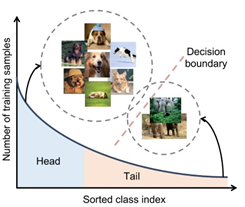
\includegraphics[width=\linewidth]{images/00_project.PNG}
  The above figure explains the data of representative reality. The horizontal axis is the type of class and the vertical axis is the amount of data 
  in each class. While pictures of dogs and cats have a lot of data, the data is bound to be small for endangered species. This distribution of data 
  is called long-tail distribution. In summary, the long-tail distribution problem is a problem in which the amount of train data for each class is not balanced.
  \newline
  \newline The biggest problem with the long-tail distribution is that instance-rich (or head) classes are mainly learned so that the model is fit into the 
  head class.\cite{kang2019decoupling} This means that the head class has high accuracy, but the tail class has low accuracy. Approaches to the Long-tail problem are largely class 
  readjustment, information augmentation, and module enhancement. Each methodology can also be divided into details, see the figure below.
  \newline  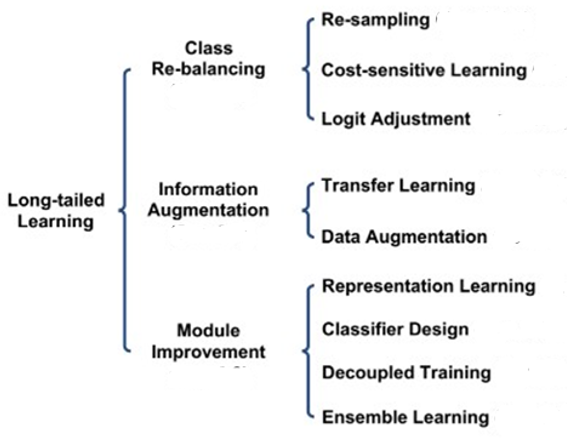
\includegraphics[width=\linewidth]{images/01_project.PNG}
  This paper deals with classifier design among class re-balancing and module improvement methods. We will also discuss how to learn models separately, an additional method of this paper, 
  compared to this method. The contribution of this paper is as follows. 
  \newline
  \newline 1) Additional ideas are added to existing methodologies to improve the performance of long-tail problems.
  \newline 2) By implementing various existing models, we take the direction of future research.
  \newline 3) We present the application form of the presented model.

\section{Related work}
  \quad As previously seen, methodologies for solving the existing long-tail problem are being studied a lot. For a rough definition of various methodologies, refer to the Deep long-tailed learning: Survey thesis.\cite{zhang2021deep} 
  This paper will describe only the models used directly in the experiment.
  \subsection{Class Re-balancing : Re-sampling}
    \quad In the long-tail problem, the number of data per classes is different. Therefore, matching the number of data per classes will be a way to solve the long-tail problem. 
    The re-sampling method is used at this time. Data augmentation techniques are sometimes used using generation models, but here, the the number of data per classes is 
    simply made equal by copying. Through this, the small the number of data per classes is over-fit because the data is repeated several times, and the large number of classes 
    is relatively under-fit. In practice, random over-smpling (ROS) and random under-sampling (RUS) are used, and to balance the class, ROS repeats the sample from the tail class 
    and RUS removes the sample from the head class. Of the two methods, the method used in this paper is the ROS method of repeating samples in the tail class. 
    That is, the amount of tail data was adjusted to be the same as the amount of head data. The limitation of this method is that the accuracy improvement is not significant 
    because the same data has been repeated. This is because it corresponds to a model that is overfitting with small data on the tail. Let's refer to the picture below.
    \newline  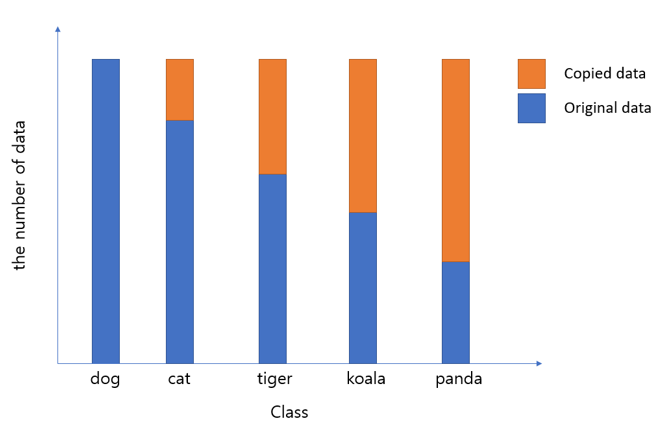
\includegraphics[width=\linewidth]{images/02_project.PNG}
    In the figure above, orange means data copied from original data. Currently, the data that actually exists is the blue part corresponding to the original data and copies 
    the original data as much as orange to match the number of data per class.
  \subsection{Moudule improvement : Classifier Design}
    \quad The next method is classifier design. Classifier design is a method of learning in consideration of the number of data per classes since the number of data per classes 
    is different when learning. For example, the value of the classifier weight to be learned is also affected by the number of data per class, so learning is carried out using 
    it appropriately. A typical example is tau-normalization To explain this, we will introduce a formula. First, let's look at the definition of the long-tail problem that will 
    be used in the future.
    \newline Long-tailed training dataset is ${\{x_i,y_i\}}^n_{i=1}$. Here, $x_i$ is data corresponding to class label $y_i$. 
    We also define the size of the entire training set as $n = \Sigma^K_{k=1}n_k$ where K is the number of classes. 
    In the case of $n_k$, it means the amount of data for class k.The mathematical definition of long-tailed learning is as follows.
    $$ if\ i_i < i_w, then \ n_{i1} \geq n_{i2}, and\ n_1 >> n_K$$
    Now, let's use the values above to learn about classifier design. For classifier design, define classifier weights W and b 
    and use the model parameter $\theta$ of the extracting the presentation step before classifier. The value passed through the classifier using this can be written as follows.
    $$W^T f(x_i;\theta) + b$$
    It is learned in the direction of minimizing the cross entropy loss between this value and the label. Here, tau-normalization modifies the value of W as follows.
    $$W_i = \frac{W_i}{||W_i||^{\tau}}$$
    However, since the accuracy of this method varies depending on the value of the tau, there is a disadvantage that a hyperparameter exists to apply it every dataset. 
    Therefore, the method that came out is Learnable Weight Scaling (LWS). This is a technique in which even the value multiplied by weight is obtained by learning. 
    If this is expressed as an equation, it is shown below and $f_i$ is learned here.
    $$W_i = f_i * w_i$$
    Here, there are several ways to learn $f_i$, and in this paper, I learned it with a model. 
    However, if this is learned separately from the parameter corresponding to the model and LWS, better results will be obtained.

\section{Approach}
  \quad Here, I will present a way to improve performance on the long-tail dataset to be presented in this paper. When writing this paper, 
  I didn't want to end up just implementing the existing method. Therefore, I tried to apply new ideas. Let's start with the beginning of the problem.
  The problem with the long-tail problem is caused by the imbalance of data. In other words, it can be expected that accuracy will increase if this imbalance is resolved to some extent.
  In other words, first, in dataset, it distinguishes between having a lot of data per class and having less data. After that, if you learn using another model, 
  the difference between the data of the most classes and the data of the least classes in the new dataset will be reduced.
  \newline  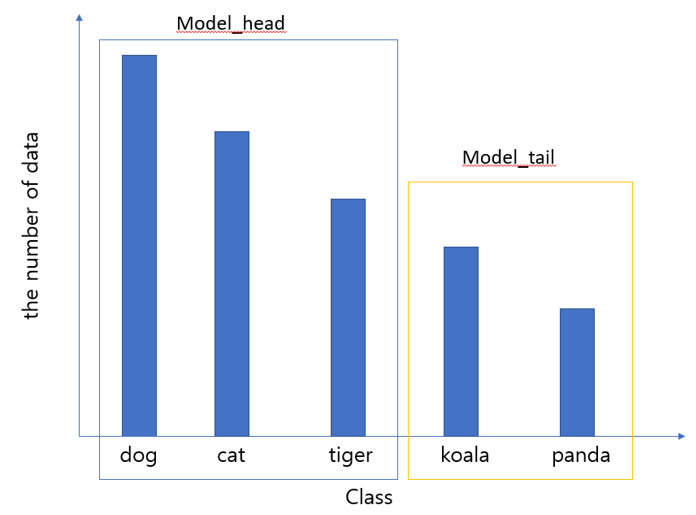
\includegraphics[width=\linewidth]{images/03_project.PNG}
  Let's take a look at the picture above. As shown in the figure above, the data gap between the head and the tail, which corresponds to the whole dataset, is significant.
  But let's make a new dataset between the data in the box to separate them into models and learn them. Let's name the two new datasets head-data and tail-data. 
  In each head-date, the difference between the amount of head data and the amount of tail data is reduced. The same is true of Tail-data. To be precise here, 
  head-data means the part where the blue box is in the figure above, and tail-data means the part where the yellow box is. 
  In this way, tail and head data also occur in two boxes, and this difference is smaller than the difference between tail data and head data amounts in the original dataset. 
  In this case, it was judged that better results could be obtained by resolving the imbalance of data.
  \subsection{Model to use in this experiment}
    \quad I will explain how to apply each of the two models with two newly created datasets by applying the above idea.
    As this model divides the dataset into two types of tail-data and head-data and learns each of the two models, 
    the training method and the test method should be applied differently. First, in the training process, learning proceeds as shown in the figure below.
    \newline  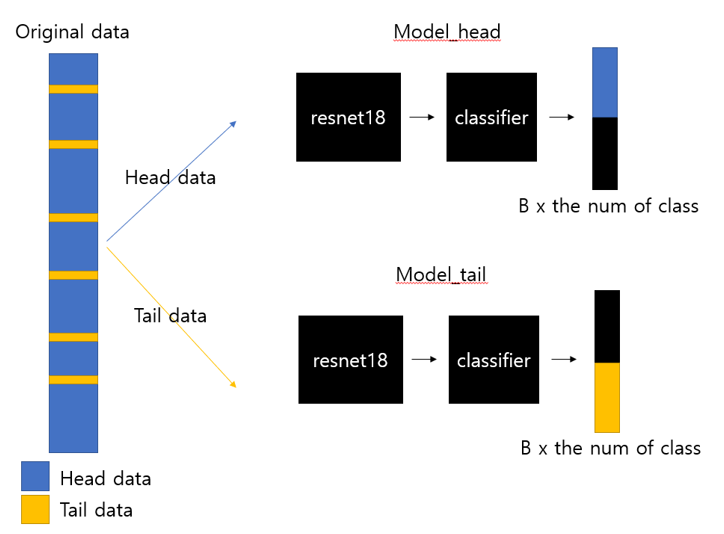
\includegraphics[width=\linewidth]{images/04_project.PNG}
    Let explain the above picture. When there is original train data, divide this data into head data and tail data. We learn the network of model head 
    and model tail, respectively, with the divided data. Then, as shown above, it will be learned so that only the colored part at the last stage has a value. 
    The reason why only these colored parts have values is that the uncolored parts are not in the dataset to be learned from the model. 
    The output obtained by combining the two learning data is now important in the test. During the test, it is shown in the figure below.
    \newline  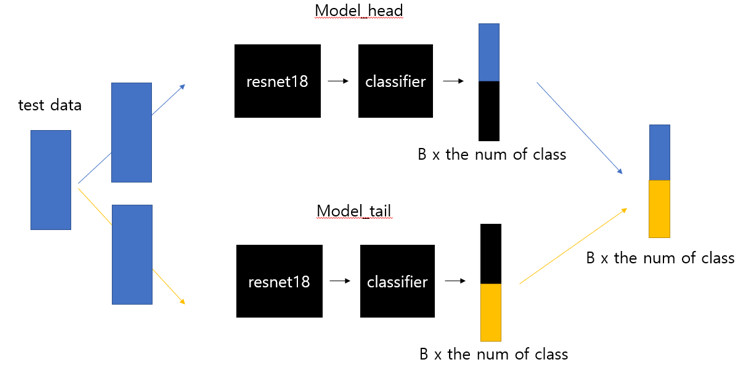
\includegraphics[width=\linewidth]{images/05_project.PNG}
    Let me explain in words. Pass the test data to two models (model head and model tail). Test data is actually a step to apply,
    and since the label of the data is not actually known, the same data must be passed through the two models. Let's look at the results 
    after the classifier passed through both data. The colored part is a valid part of each model. For example, each data value looks like this:
    \newline  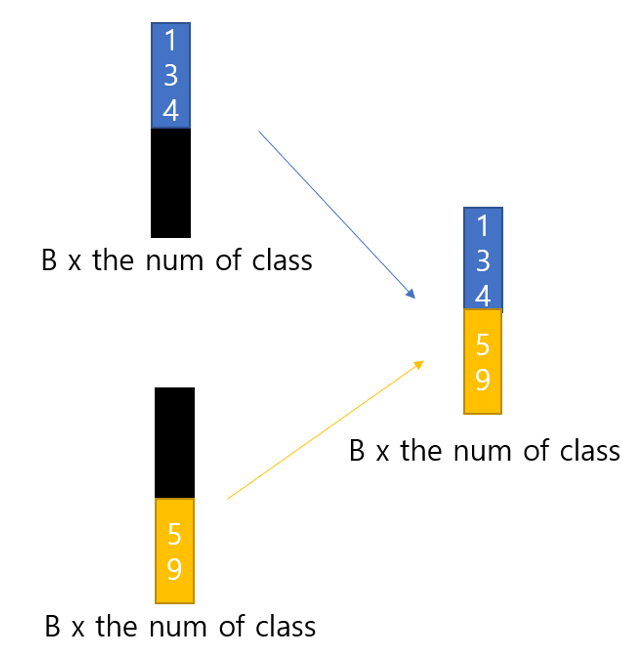
\includegraphics[width=7cm]{images/06_project.PNG}
    \newline If you simply add it up to the value as above, you will eventually be able to obtain an index corresponding to 9 as a predicted label value. 
    Although it is not too much to proceed with learning in this way, I think that better results will be obtained by dividing the sum of each output 
    when combining the outputs from the two models. The method I just mentioned is as follows.
    \newline  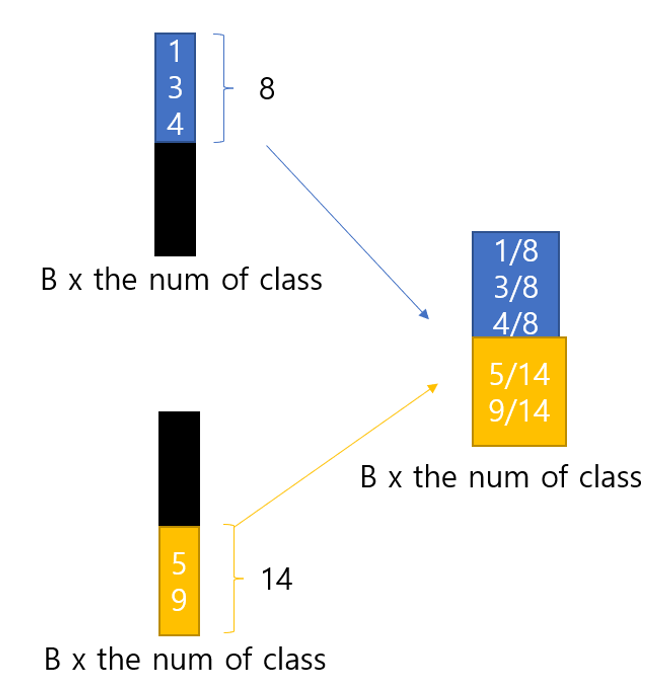
\includegraphics[width=7cm]{images/07_project.PNG}
    \newline What to consider with this data model is how to divide the data set. In this experiment, Dataset is sorted in descending order by the amount of data per class. 
    After that, it was divided into new dataset based on half of the class number. The method described here is shown in the figure below.
    \newline  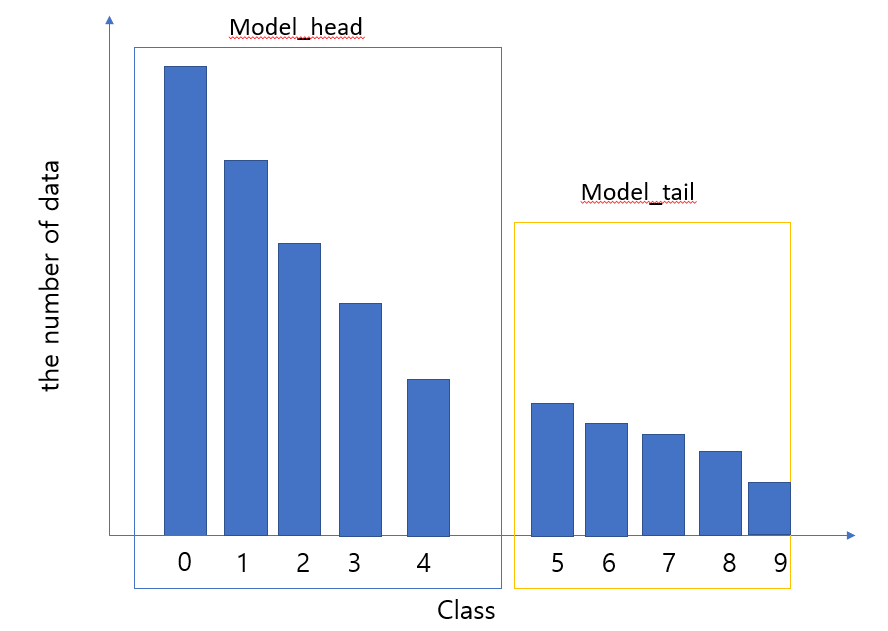
\includegraphics[width=\linewidth]{images/08_project.PNG}
  \subsection{Additional Thinking Models}
    \quad In fact, it can be designed without a black part, but in order to use the given baseline code as much as possible, it was designed as above. 
    In this section, we will explain additional models that can be tested. This method divides original data equally into head data and tail data. 
    There is a difference after that, and I will start with how to train model-head. Leave the label of the head data to learn from the head-model. 
    And change the labels of the tail data to the same new value. I hope the picture below is helpful for your explanation. 
    You want to consolidate the tail data into one label and recognize the value as data that does not correspond to the head data. 
    Because the number of tail data is relatively small, data balancing is performed by making them all one label.
    \newline  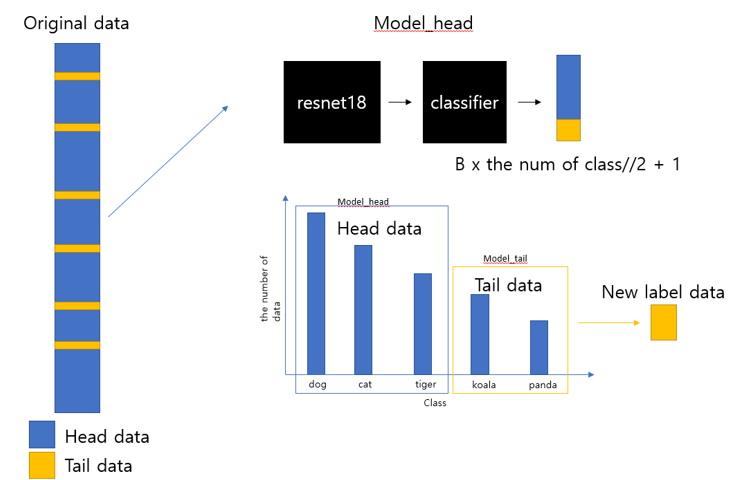
\includegraphics[width=\linewidth]{images/09_project.PNG}
    Next, let's look at tail-model. In the case of tail-model, it is almost the same, but if all head data are unified into one label, the data unbalancing problem appears. 
    Therefore, it must be matched to the average value of the amount of tail data or to the smallest amount of data or the largest amount of data. Let's refer to the picture below
    \newline  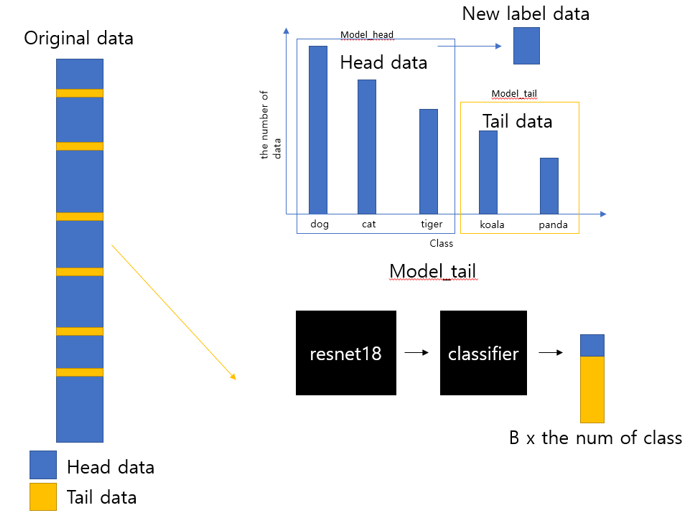
\includegraphics[width=\linewidth]{images/10_project.PNG}
    In the test, the learned method is output by combining the results derived from model-head and model-tail like the model presented at the beginning.
    I have a few questions about the performance of this model. First, for example, the model learns dogs, cats, and tigers from their respective labels, 
    but all other data must be learned from the same label. It is a question of whether this will work out. In other words, 
    it is a question of whether it is possible to learn a model that recognizes panda and koala data with the same label. 
    Second, it will take more time because not only do you have to change all the data labels on the train, but you also have to learn both the head and tail models of the data.
    \newline So we used the first model in this paper's experiment. But I think the second model is also expected to press better performance if the first one of the problems presented above goes well.

\section{Experiment} 
  \subsection{Dataset}
  \quad This experiment was conducted on a total of 8 datasets. The basic framework used CIFAR dataset. This CIFAR10 dataset is reduced to 10 classes, and CIFAR100 is set to 100 classes.
  And the util given to baseline. Data unbalancing will be performed using functions IMBALANCECIFAR10 and IMBALANCECIFAR100 in utils.py. 
  In this case, there is a way to change the method to step and exponential. And at this time, 0.1 and 0.01 are given as unbalancing factors, so learning can be conducted in a total of 8 datasets.
  \begin{table}
    \centering
    \caption{Dataset}
    \label{t1}
    \begin{tabular}{|c|c|c|c|}
    \noalign{\smallskip}\noalign{\smallskip}\hline
    & dataset & IMB-TYPE & IMB-FACTOR \\
    \hline
    dataset1 & CIFAR10 & exp & 0.1 \\
    \hline
    dataset2 & CIFAR10 & exp & 0.01 \\
    \hline
    dataset3 & CIFAR10 & step & 0.1 \\
    \hline
    dataset4 & CIFAR10 & step & 0.01 \\
    \hline
    dataset5 & CIFAR100 & exp & 0.1 \\
    \hline
    dataset6 & CIFAR100 & exp & 0.01 \\
    \hline
    dataset7 & CIFAR100 & step & 0.1 \\
    \hline
    dataset8 & CIFAR100 & step & 0.01 \\
    \hline
    \end{tabular}
  \end{table}
  Table 1 shows the number of eight cases.
  Dataset was especially used by dividing it into test dataset and validation dataset. The way to divide is the 'random\_split' function of 'torch.utils.data' was used.
  \subsection{Implementation}
  \quad The experimental environment was conducted in pytorch. The GPU also used the NVIDA GeForce RTX 3060 Ti. ResNet 18 was used as a model. 
  This model will be baseline. The model implementation methods include Re-sampling, classifier design using LWS, and a method of separating the model proposed in this study.
  In this method, it was divided into test dataset and validation dataset. In addition, CrossEntropyLoss was used as the loss, SGD was used as the optimizer.
  The use of Scheduler used StepLR. Other factors are as follows.
  The following figure shows the label values and images of dataset1. What Tensor 3 means is label and below it is image data.
  \newline momentum = 0.9
  \newline learning rate = 0.1 
  \newline weight decay = 2e-4
  \newline Batch size = 128
  \newline step size = 150
  \newline gamma = 0.1
  \newline  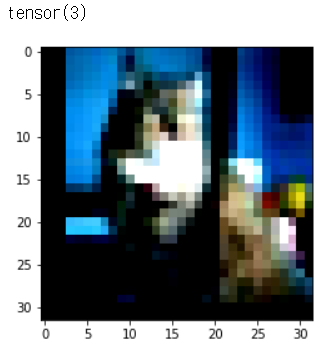
\includegraphics[width=6cm]{images/11_project.PNG}
  \subsection{Result}
  \quad The result in Table 2 to be examined first is the result of the experiment conducted to examine the approximate tendency.
  %, and the dataset did not divide the validation and test. 
  Through this experiment, we were able to decide which method to use. This experiment used dataset1 in common.
  From the results of Table 2, it can be seen that the model improved the performance of tail and head precision by my model and LWS technique. 
  The reason why the head and tail have risen is that for two models that have learned only head and tail data, there are fewer cases where the weight changes 
  due to different data on the labels.
  \begin{table}
    \centering
    \caption{tendency}
    \label{t1}
    \begin{tabular}{|c|c|c|c|}
    \noalign{\smallskip}\noalign{\smallskip}\hline
    & Accuracy & Head Accuracy & Tail Accuracy \\
    \hline
    Baseline & 67.52 & 73.42 & 61.62 \\
    \hline
    Re-sampling & 72.91 & 74.94 & 70.88 \\
    \hline
    LWS & 67.40 & 72.84 & 61.96 \\
    \hline
    my model + LWS & 80.36 & 80.56 & 80.16 \\
    \hline
    \end{tabular}
  \end{table}
  \newline
  \newline For reference, in the case of model isolation, compute\_accuracy was applied to two models in the accuracy measurement, and head\_acc was calculated 
  by taking head\_acc from model\_head and tail\_acc from model\_tail. This is possible because the compute\_accuracy is designed to extract only each value. 
  Let's refer to the picture below.
  \newline  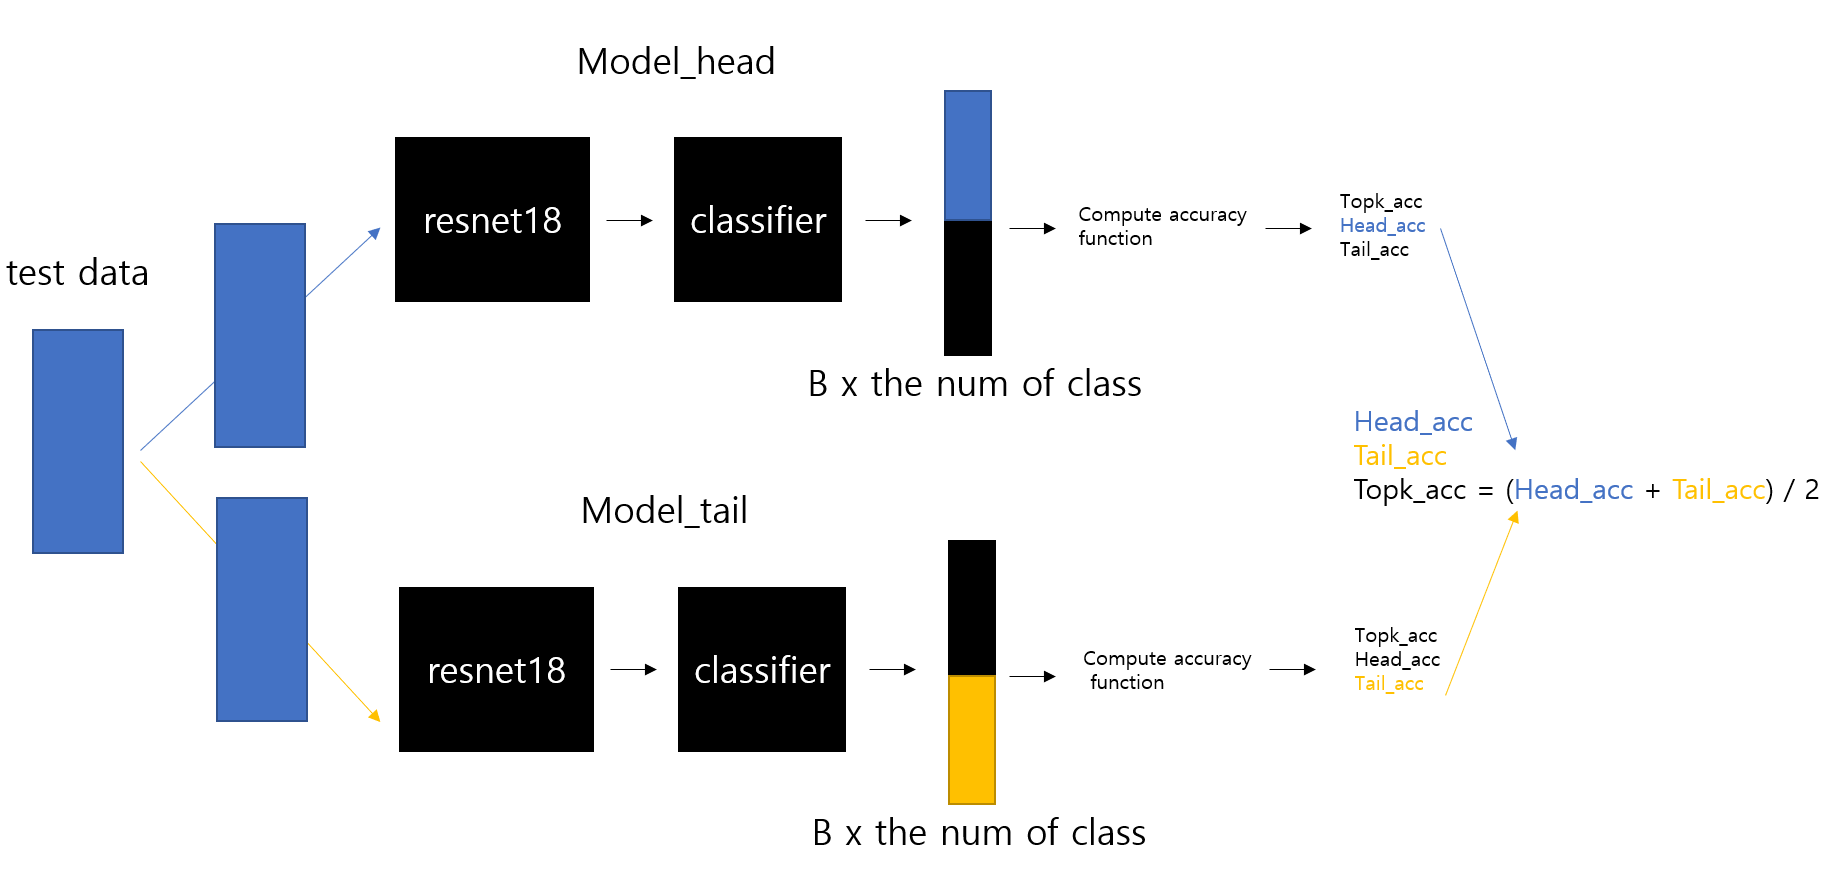
\includegraphics[width=\linewidth]{images/12_project.PNG}
  The reason for this is that the current test data set has a label and is also designed so that the compute\_accuracy function is calculated separately. 
  Therefore, in order to check the performance of this model, you can use it in the same way as above. To apply data without an actual label, 
  the method mentioned in the appoach section can be used. The criterion for dividing the validation dataset and the test dataset was 9:1.
  \newline
  \newline Through the first experiment, it was confirmed that model separation was effective. In addition, in the experiment to be conducted from now on, 
  the gradient clipping technique was also applied to the model. This is because in the case of mymodel, the gradient value was infinite at model-tail and pred was nan at model-tail. 
  Since validation and test were divided by random split, there is a difference between the above result value and the below result value. 
  The parameter used in the results below is the same as the value described in the implementation above.
  \newline 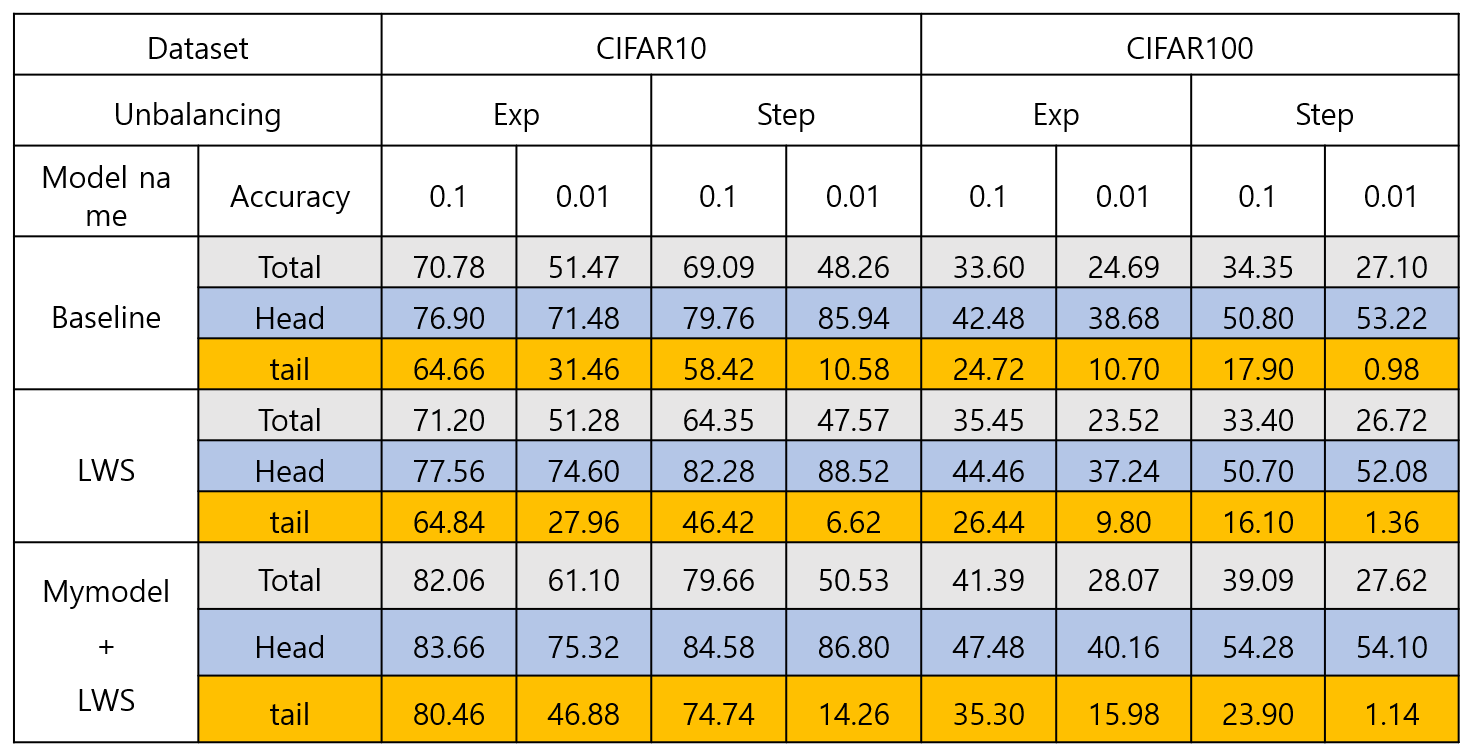
\includegraphics[width=\linewidth]{images/13_project.PNG}
  When analyzing the above results, the total value was superior to the reference value of the 'my model + LWS' model. In particular, 
  the accuracy of the tail increases, showing better performance. However, when using only LWS, the entire data is not only learned from one model, 
  but is often lower than the baseline because the epoch is 100. This value, which LWS multiplies the weight of the classifier, has not yet been properly learned, 
  as described in the relevant study. On the other hand, in the case of "My Model+", the "LWS" model and the epoxy are small, but the data class is reduced in half, 
  making it possible to judge that the learning was well done. In order to confirm that the above situation was correct, 
  the learning was conducted by extending the epoch to 200. Only dataset 5 was used at this time was used.
  \newline 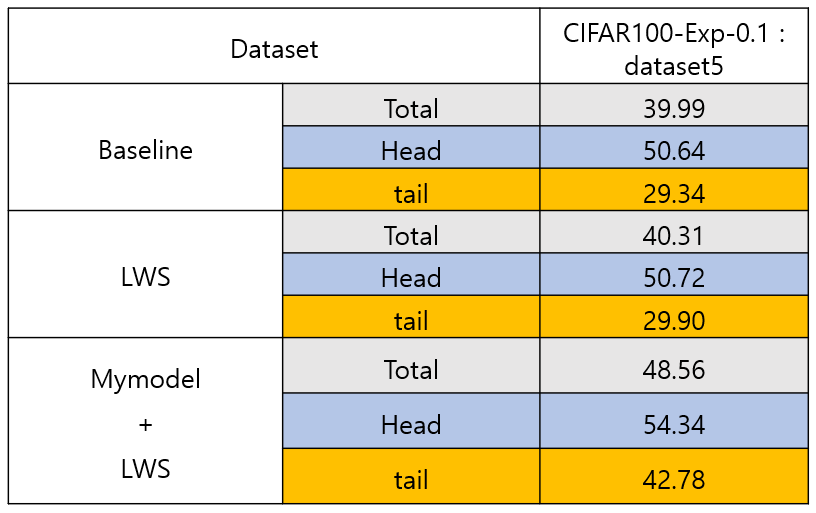
\includegraphics[width=\linewidth]{images/14_project.PNG}
  As you can see, as the epoch increased, the performance of all models increased. However, in the case of LWS, there was no significant difference compared to baseline. 
  As mentioned in Related work, it seems that better results can be obtained only when LWS is additionally fine-tuned with the data learned first.
  \subsection{Training/test time consumption}
  \quad This time we will look at the execution time. To compare the execution time, the execution time was compared on the same GPU. 
  The GPU used the NVIDA GeForce RTX 3060 Ti. The results show that my model has a long execution time.
  \newline 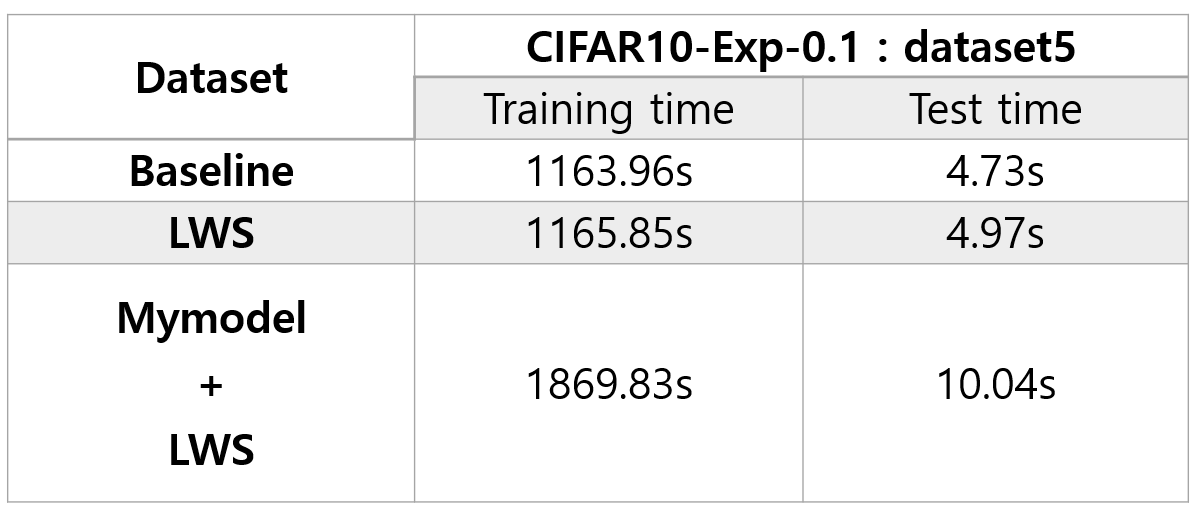
\includegraphics[width=\linewidth]{images/15_project.PNG}
  \subsection{Some example images}
  This experimental result predicted the prediction result by applying the method of predicting the real model described in approach.
  \newline 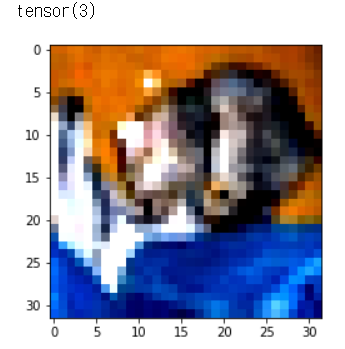
\includegraphics[width=6cm]{images/16_project.PNG}
  \newline Looking at the figure above, the tensor 3 value means target. Let's see if we can predict these results.
  The image is passed through the model\_head and model\_tail, respectively, and the pred\_head and pred\_tail values are obtained. After that, 
  5 values in front of the pred\_head and 5 values after the pred\_tail are concatenated to make a pred. If you find an index with a maximum value using Torch.
  argmax, you can obtain a tensor 3 as shown below.
  \newline 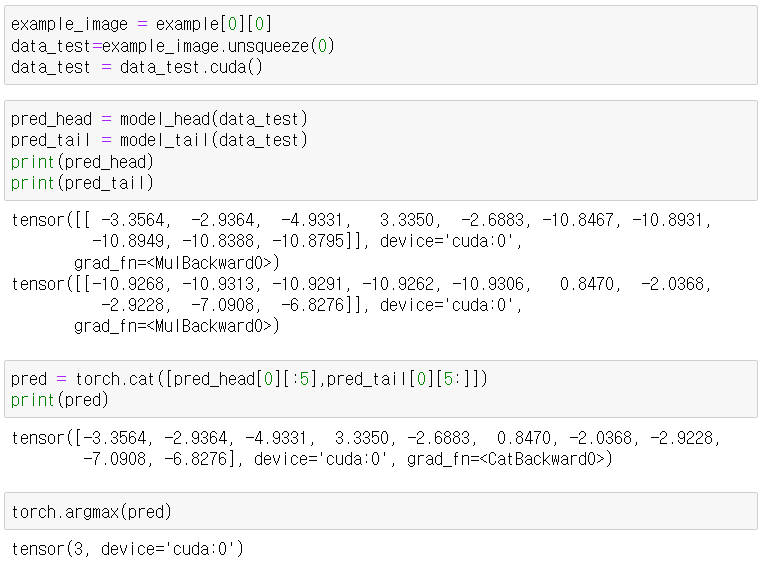
\includegraphics[width=6cm]{images/17_project.PNG}
  \newline Let's look at one more successful case.
  \newline 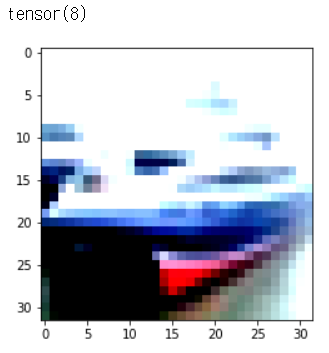
\includegraphics[width=6cm]{images/18_project.PNG}
  \newline 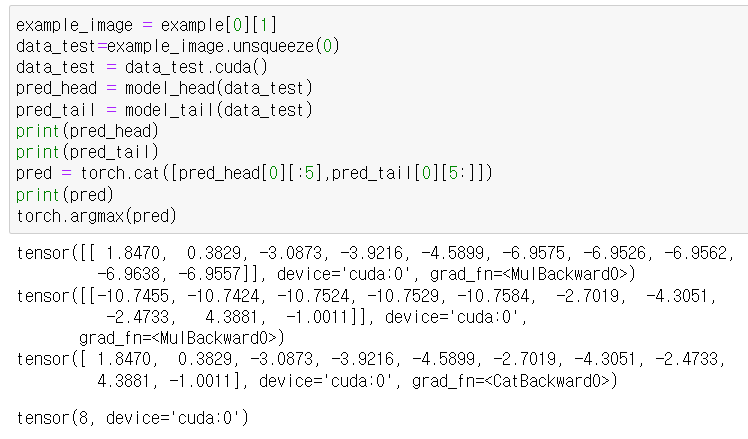
\includegraphics[width=6cm]{images/19_project.PNG}
  \newline This time, let's look at the failed case.
  \newline 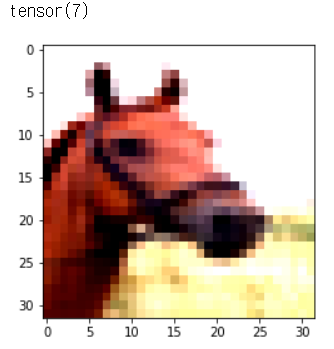
\includegraphics[width=6cm]{images/20_project.PNG}
  \newline 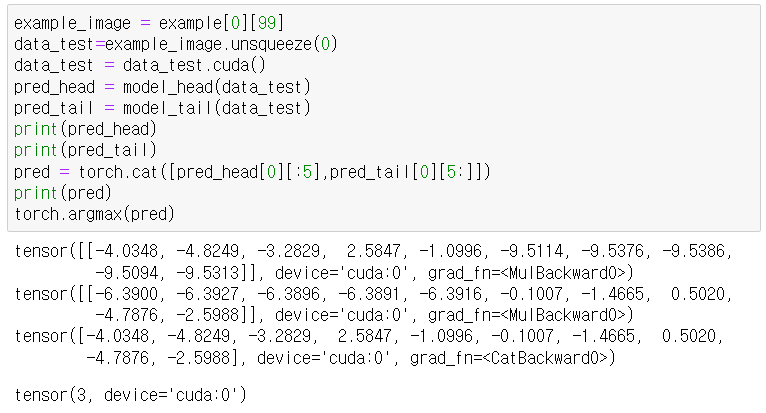
\includegraphics[width=6cm]{images/21_project.PNG}
  \newline Let's look at why the above results failed. The maximum value of the first five values in the pred\_head is 3. 
  On the other hand, index 7 is the maximum value of the last five values in pred\_tail. 
  However, since the value of index 3 is larger, it can be seen that it is expected to be 3.
  To mitigate this difference, let's calculate it after dividing it by the sum of the absolute values that I thought of.
  \newline 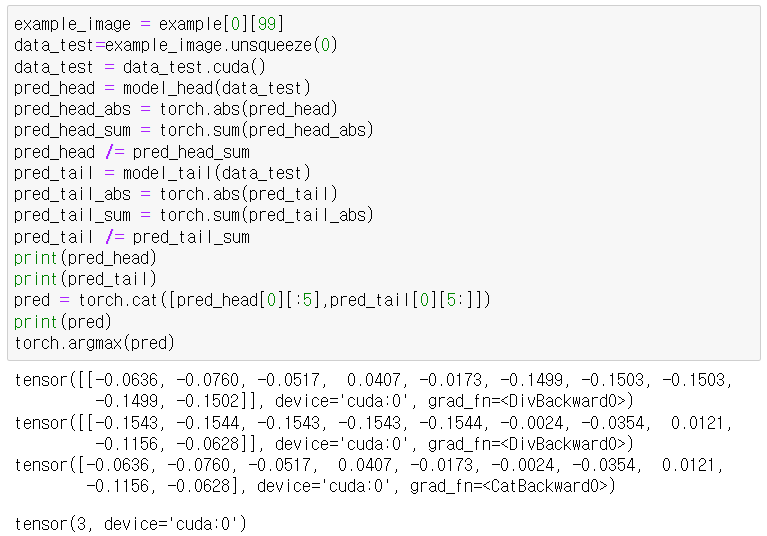
\includegraphics[width=\linewidth]{images/22_project.PNG}
  Although the difference in value has decreased, it is still expected to be 3. Therefore, it seems necessary to think about how to solve this error later.





\section{Conclusion}
  \quad The long-tail problem is a problem raised to apply deep learning well to real data. In this paper, we look at how to improve performance on datasets of Long-Tail distributions. 
  Basically, the LWS technique was used, and the performance was shown to be improved by defining a new model. The new model is a method of dividing data sets to learn the model. 
  Each of these divided datasets is trained on a different model.
  \newline 
  \newline Future research is to design the model proposed in this study practically. This study has shown that performance improvements are possible, but nevertheless, 
  details have not yet been designed. 
  \newline
  \newline First, in this study, we divided the data set by half the number of classes as a basis for segmentation. 
  In this work, we were able to meet this criterion well because we made the dataset unbalanced using defined functions. However, physical data may not. 
  Therefore, research on how to split the data set should be carried out.
  \newline
  \newline Second, in this study, the accuracy measurement did not proceed with the appropriate sum of the output of the model\_tail and model\_head proposed by approach section. 
  In the project, I derive that accuracy increases by properly using the compute\_accuracy, which is designed as a given code. In order to be used elsewhere, 
  it is necessary to combine the outputs from the two models. Since the design method has already been presented, 
  it is necessary to design it so that the results can be produced properly in the test set.
  \newline
  \newline Third, since the gradient clipping technique was used in this study, the results vary depending on the hyperparameter max\_num value. 
  The reason for using this technique is that when learning a model with tail\_dataset separated from a dataset, gradient values often have infinite values, 
  causing the model to break down. However, in this study, max\_num was simply designed as 5, and it is necessary to apply it appropriately through a clearer 
  understanding of the concept.
  \newline
  \newline The last thing I thought about was that in this study, the dataset was divided into two, but I think it can be divided into smaller pieces.

\section{Appendix}
  This experiment is conducted with various models, so there are too many files. So I would like to explain to help you understand.
  \newline
  \newline First, the file 'DLLAB\_project\_baseline.ipynb' is the file used to learn the baseline model, and the log file is stored in the log/baseline. 
  For accuracy, you can read the log model from the file 'DLLAB\_project\_baseline.ipynb', but you must run the log model one after another to generate the test data set. 
  This means that the code must be executed before the learning code line and then moved to the next load. 
  In addition, the name of the DATASET should be changed to CIFAR10 and CIFAR100 depending on the model to be called for the test dataset.
  \newline
  \newline The second file is the 'DLLAB\_project\_tendency.ipynb' file. This file is the file used to create Table 2, and contains the results of each model's dataset1. 
  Here, the accuracy measurement method is the same except for mymodel.
  \newline
  \newline The third is the 'DLLAB\_project\_LWS.ipynb' file. This file is a file created to examine the results when learning by applying the LWS technique, 
  and the model can be retrieved and checked in the same way as 'DLLAB\_project\_baseline.ipynb'. 
  The results were not very good, but it seems that it was difficult to produce meaningful results 
  because the data learned by dividing the data set into train and validation data set was reduced.
  \newline
  \newline The last file is the 'DLLAB\_project\_mymodel.ipynb' file. This file contains the results of learning by applying the method introduced in the above study. 
  This can also be checked by calling the model in the same way as 'DLLAB\_project\_baseline.ipynb'.






\newpage
\bibliography{egbib}
\end{document}